\documentclass{deimj}
\usepackage[dvipdfmx]{graphicx}
%\usepackage{latexsym}
\usepackage{txfonts}
%\usepackage[fleqn]{amsmath}
%\usepackage[psamsfonts]{amssymb}
%\usepackage[deluxe]{otf}

% 印刷位置調整 %
% 必要に応じて値を変更してください.
\hoffset -10mm % <-- 左に 10mm 移動
\voffset -10mm % <-- 上に 10mm 移動

\newcommand{\AmSLaTeX}{%
 $\mathcal A$\lower.4ex\hbox{$\!\mathcal M\!$}$\mathcal S$-\LaTeX}
\newcommand{\PS}{{\scshape Post\-Script}}
\def\BibTeX{{\rmfamily B\kern-.05em{\scshape i\kern-.025em b}\kern-.08em
 T\kern-.1667em\lower.7ex\hbox{E}\kern-.125em X}}

\papernumber{DEIM Forum 2014 F1-6}

\jtitle{プレゼンテーションスライドに対する分割手法の提案と\\講義スライドへの応用}
%\jsubtitle{サブタイトル}
\authorlist{%
 \authorentry[sakamoto@db.soc.i.kyoto-u.ac.jp]{坂本 祥之}{Yoshiyuki SAKAMOTO}{kyotou}% 
 \authorentry[tshimizu@i.kyoto-u.ac.jp]{清水 敏之}{Toshiyuki SHIMIZU}{kyotou}% 
 \authorentry[yoshikawa@i.kyoto-u.ac.jp]{吉川 正俊}{Masastoshi YOSHIKAWA}{kyotou}% 
}
\affiliate[kyotou]{京都大学大学院情報学研究科\hskip1zw
  〒606--8501 京都府京都市左京区吉田本町}
 {}


%\MailAddress{$\dagger$hanako@deim.ac.jp,
% $\dagger\dagger$\{taro,jiro\}@jforum.co.jp}

\begin{document}
\pagestyle{empty}
\begin{jabstract}
近年,学会での発表や,講義などで,プレゼンテーションスライドが使われることが増えている.
その中で,講義のプレゼンテーションスライド(以下,「講義スライド」と呼ぶ)は,講義を欠席した人や,後で講義を復習したい人のために,公開されていることも多い.
しかし,講義スライドは,講義を聞くことを前提として作られている場合など,そのままでは理解できないことも多い.
本研究では,話題ごとに講義スライドを分割(セグメント化)することで,講義スライドの閲覧を補助することを考える.
また,セグメント情報を利用して,様々な講義を比較するといった応用例についても考察する.
\end{jabstract}
\begin{jkeyword}
プレゼンテーションスライド
\end{jkeyword}
\maketitle










\section{はじめに}

近年,学会の発表や学校の講義で,Microsoft PowerPoint 等のソフトウェアで作成された,プレゼンテーションスライドが広く使われている.
特に,講義スライドに関しては,講義の復習のためや,講義に出席できなかった人のために,配布されたり,公開されることも多い.
スライドは,教科書等に比べて,図や表が多く,文章が少ないため,講義の概要が知りたい場合や,直感的な理解をしたい場合に有用である.
しかし,プレゼンテーションスライドは,口頭発表することを前提として作成されている等の理由により,それ単体では内容を理解できないことも多い.

本研究では,まず,プレゼンテーションスライドを,話題毎に分割する方法を提案する.
1つのプレゼンテーションスライドには,複数の話題が含まれることがある.
そのため,スライドに含まれる文字情報を用いることで,
プレゼンテーションスライドを,同じ話題について述べている部分に分割する.
この部分を``セグメント''と呼ぶ.
3章では,まず,先行研究について述べる.
これは,単語とインデントの情報から,セグメント分割を行うという手法である.
さらに,先行研究の改善点として,tf-idfで単語の重み付けをするなど,セグメント分割の精度を改善する手法について述べる.

次に,今回の手法の講義スライドへ応用について述べる.
講義は,異なる大学で同じ内容について行っていることも多いため,
自分の大学と他の大学の講義を比較する,といったことが考えられる.
講義スライドへの応用については,4章で詳しく述べる.

% \begin{verbatim}
%  \papernumber{DEIM Forum 2014 XX-Y}
% \end{verbatim}










\section{関連研究}

プレゼンテーションスライドからの情報取得や,検索等についての関連研究として,以下の研究が挙げられる.

羽山ら\cite{hayama2008} \cite{hayama2009}の研究では,1枚のスライド内の構造化を行なっている.
スライド内の配置の情報とフォントの情報から,スライド内のオブジェクトを,タイトル,本文,図,表,装飾という5つに分類し,一枚のスライド内の情報を木構造で表現している.

さらに,羽山らの別の研究\cite{hayama2010}は,\cite{hayama2009}の手法をベースとして,検索要求に関連する箇所だけを抽出し,提示する手法を提案している.

北山ら\cite{kitayama2009}の研究では,スライド間の関係を求めている.
この研究では,スライドの単語と,そのインデントの情報,発表テキストをデータとして利用している.
スライド間の関係としては,詳細化,汎化,具体化,付加の4種類を定義している.
ある基点スライドを決め,そのスライドに出現している一つの単語着目し,基点スライドと関係のあるスライドを求め,関係を分類している.
基点スライドが同じでも,着目する単語が違うと,関係が異なる場合がある.
%我々は発表ビデオは利用せず,プレゼンテーションスライドのみを使って行っているが,単語やインデント等の利用については,この研究をベースとしている.
%ため,この研究をベースに,少し異なった手法を取る必要がある.

王ら\cite{wang2010}の研究では,北山らのような,インデントを利用した表層的構造に加えて,WordNetを利用し,語のIS-A関係やPART-OF関係による概念的構造を求め,その両方を利用することにより,スライド間の関係を求めている.

別の王ら\cite{wang201009}の研究では,表層的構造から,スライド間の関係を Detailed と Generalized に分類している.
さらに,ユーザが入力するキーワードについて良く知っている場合のDETAIL検索と,あまり知らない場合のGENERALITY検索の2種類を考え,スライドのランキングを行なっている.
%我々の研究では,単語の概念的構造は考えていないが,1枚あたりの記述が少ないスライドにおいて,このような概念構造を利用するのは有用であると考えている.

Vinciarelliら\cite{vinc2006}の研究では,スライドの画像からから,文字認識をすることにより,スライドからテキストの抽出を行なっている.
さらに,スライドは,1枚に含まれるテキストの量が不均一であるため,テキスト量に依存しないtf-idf法を考案し,入力されたキーワードに対して,スライドをランキングする手法を提案している.
%我々の提案手法の応用として検索システムを構築する場合,利用できる部分がある.

Atapattuら\cite{atapattu2012}の研究では,プレゼンテーションスライドに出現する単語の重み付けを行なっている.プレゼンテーションスライドのテキストとその装飾情報を抽出し,利用している.単語の出現頻度と,その装飾,その単語が長文中に出現しているか短文中に出現しているかという3つ情報を使い,単語に重みをつけている.
% また,装飾情報から,概念や概念間の階層関係を抽出しているらしいが,ここはまだ理解できていないので省いている
% 我々の研究では,テキストの装飾情報は利用していないが,装飾の情報は,論文等他の文章には無い特徴である.単語の重み付けをする際に,装飾情報を考慮するのであれば,この研究の手法が利用できるのではないかと考えられる.

田中ら\cite{tanaka2012}の研究では,プレゼンテーションスライドのテキスト部のみを対象としている従来の検索の手法に対し,図形やイラストの形状や配置を考慮したプレゼンテーションスライドの検索手法を提案している.
プレゼンテーションスライドは,論文等に比べて,テキストが少なく,画像や図形が多く使われるため,その形状や配置は重要な情報になると考えられる.
%また,我々の研究の応用として,プレゼンテーションスライドの検索システムを構築する場合,この田中らの研究の手法は参考にできる.

友安ら\cite{tomoyasu2012}の研究では,研究発表において,プレゼンテーションスライドを素材として作られたポスターの閲覧支援システムを構築している.
ポスターは,一見しただけではどこから見るべきか分からないため,スライドのポスターの対応付けを行い,スライドの順序にもとづき,ポスターの閲覧順序を決定する.
スライドとポスターの対応付けを行う際には,インデントの情報からそれぞれの構造情報を取得し,テキストの類似度と構造の類似度の両方の算出を行なっている.

% Kan \cite{minyen2007}の研究では,学会発表のプレゼンテーションスライドと,それに対応する論文の,部分同士の対応付けを行なっている.
% 我々の研究では,プレゼンテーションスライド単体からの構成抽出を考えているが,対応する論文が存在する場合,論文との対応付けをとり,論文の構造を見ることでプレゼンテーションスライドの構造を抽出する手法も考えられる.

山田ら\cite{yamada1999}の研究では,技術論文の内容からシナリオを作成し,プレゼンテーションスライドの構成支援をする手法を提案している.
%我々の研究でも,作成したプレゼンテーションスライドを入力として,スライドが正しく構成されているかをチェックするといったアプリケーションを作成することも可能であると考えられる.例えば,目次スライドと実際の構成が異なっていることを見つけて,作成者に注意を促す等が考えられる.

Tajimaら\cite{tajima1998}の研究では,メールの返信や,ウェブニュースのコメント返信,HTMLのリンクのような,
木構造で表される文書集合について,同じトピックを述べているコメントや,ページの集合を求めている.
% HTMLのリンク構造等を木構造で表し,ノード間の類似度については,単語ベクトルのコサイン類似度を用いている.
% ノードの捜査の順番や,トピックの重複を許すなどの要素を含んでいる.

岡本ら\cite{okamoto2004}の研究では,講義のプレゼンテーション資料や,
動画といった教育コンテンツに対する高度な検索機能を実現するUPRISEというシステムを提案し,
tf-idfや,前後のスライドの関係などを考慮した検索を行う手法について述べている.

Wangら\cite{wang2013}の研究では,スライドから Word Cloud を抽出することにより,
プレゼンテーションスライドの Quick Browsing を可能にする手法を提案している.
この研究では,スライドのContextという概念を定義し,それに基づき,単語を重み付けしている.
そして,その重みによって単語のフォントサイズを変更し,スライドのタグクラウドを生成している.







\section{スライド分割手法}

本章では,まずセグメントについて説明し,
我々の先行研究 \cite{sakamoto2013}について説明する.
そして,その後,本研究での手法改善について説明する.

\subsection{セグメントについて}

セグメントとは,プレゼンテーションスライドの中で,共通の話題について述べている部分である.
一つのプレゼンテーションスライドには,一般的に,複数の話題が含まれる.
そのため,まずはプレゼンテーションスライドを話題ごとにセグメントに分割する.
例えば,プレゼンテーションスライドPの中で,話題A,話題B,話題Cが述べられていたとすると,
Pは,図\ref{fig:segment}(1)のように,三つのセグメントに分けられることになる.

セグメントについては,スライドの連続性を考慮し,本稿では,
図\ref{fig:segment}(2)のような,隣り合っていない,離れたスライドが,他のセグメントを飛び越えて一つのセグメントにはならないと仮定する.
また,単純化のため,セグメントは,図\ref{fig:segment}(3)のような階層のような構造を持たず,セグメントを含むセグメント等は定義しないことにする.

\begin{figure}[tb]
 \begin{center}
  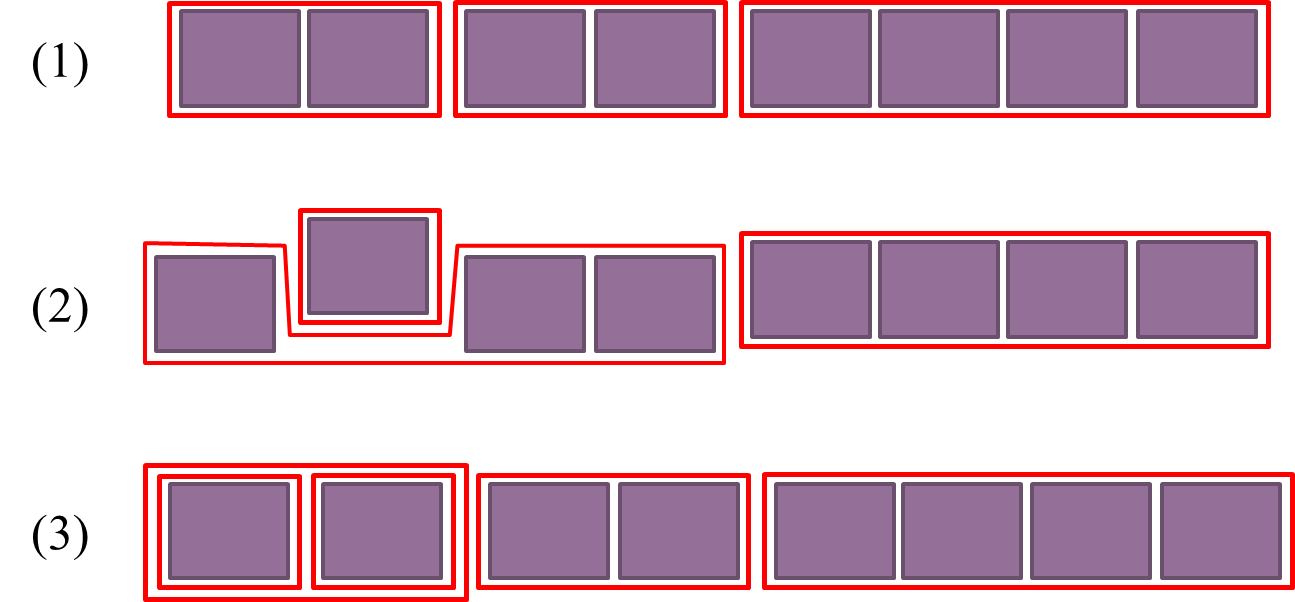
\includegraphics[width=80mm,height=40mm]{slide_segment.png}
 \end{center}
 \caption{セグメント}
 \label{fig:segment}
\end{figure}


\subsection{先行研究}\label{subsec-exist}

セグメント分割手法は,我々の先行研究 \cite{sakamoto2013} の手法手法を元に,
手法の改善を行ったため,まずは先行研究の手法の説明を行う.

\subsubsection{スライドから取得する情報}\label{subsubsec-word}

先行研究では,スライドから,単語と,その単語の出現しているインデントの位置を抽出した.インデントについては,以下のように定めている.

\begin{itemize}
 \item タイトルを最上位であるインデント0とする.
 \item 本文の最上位のインデントを1とし,以下インデントされる度に2,3,... とする.
 \item インデントの情報が含まれていないテキストについては,``インデント情報なし'' とする.
\end{itemize}

\begin{figure}[tb]
 \begin{center}
  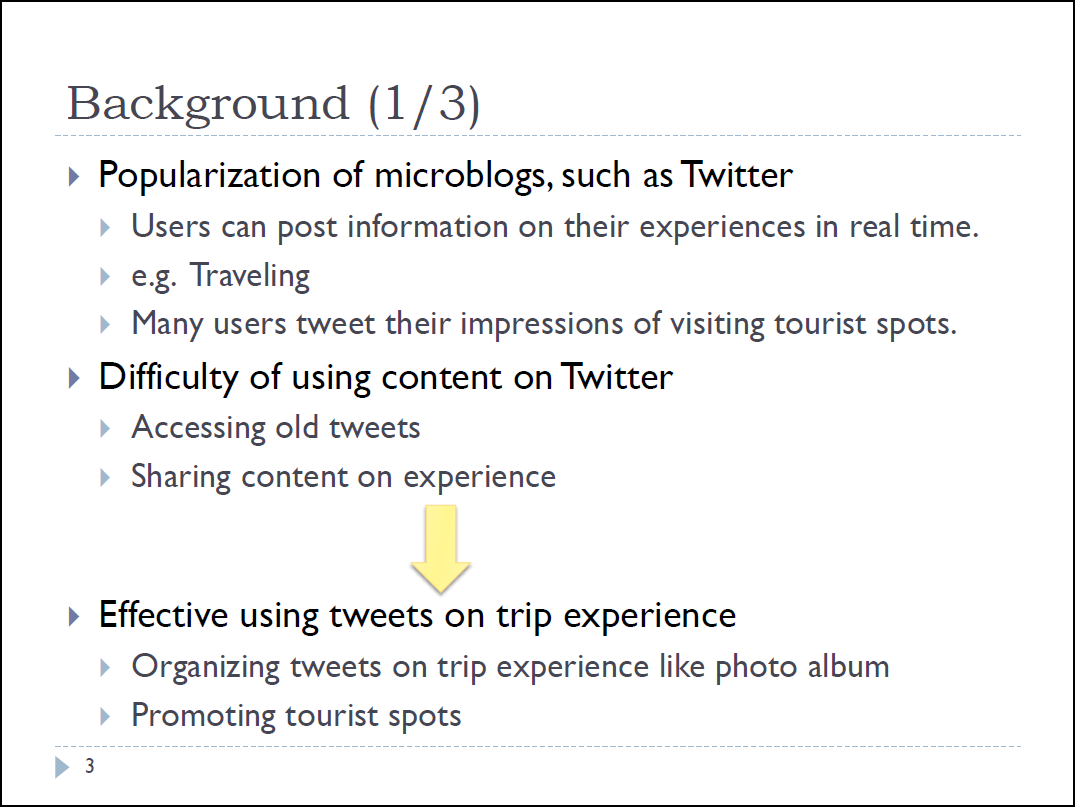
\includegraphics[width=64mm,height=48mm]{slide.png}
 \end{center}
 \caption{スライドの例}
 \label{fig:segment}
\end{figure}

\subsubsection{目次スライドとスライドの場合分け}

プレゼンテーションスライドには,目次スライドが含まれている場合がある.
目次スライドとは,例えば,図\ref{fig:outline}のようなものである.

図\ref{fig:outline}のような目次スライドがあった場合に,後のスライドには,``Background''や,``Related Work''というタイトルのスライドが続くことが多い.

目次スライドの出現パターンから,プレゼンテーションスライドは,以下の3種類に分類できる.

\begin{figure}[b]
 \begin{center}
  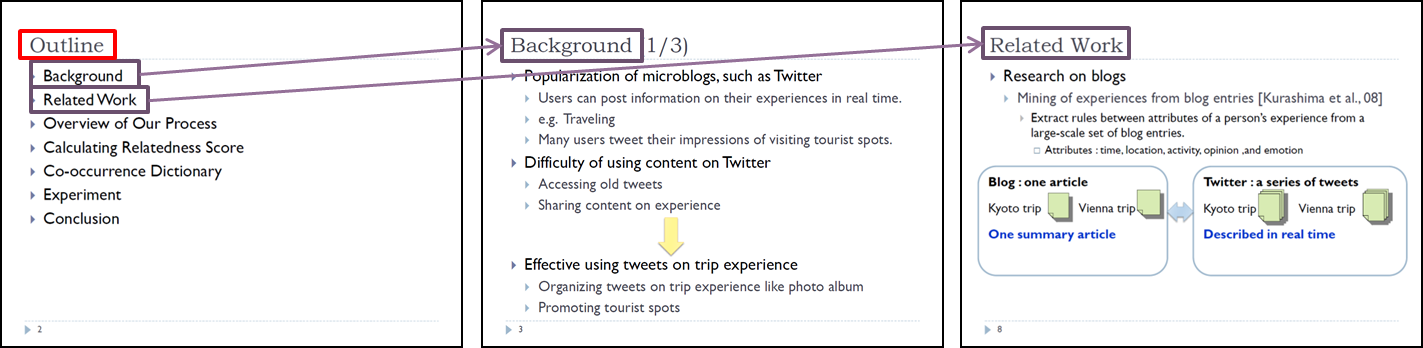
\includegraphics[width=80mm,height=20mm]{outline.png}
 \end{center}
 \caption{目次スライドの例}
 \label{fig:outline}
\end{figure}

\begin{itemize}
 \item {\bf 複数目次}\\
  プレゼンテーションスライドの中に,目次スライドが複数含まれている場合である.
一つの話題が終わる度に目次スライドをはさみ,今発表している箇所を把握しやすいようにしている場合である.
 \item {\bf 単一目次}\\
  プレゼンテーションスライドの序盤に1枚だけ目次スライドが含まれる場合である.
 \item {\bf 目次なし}\\
  プレゼンテーションスライドに目次スライドが含まれていない場合である.
\end{itemize}

複数目次のプレゼンテーションスライドについては,一つの話題が終わるごとに目次スライドを挟むのが普通である.
よって,目次スライドから目次スライドまでを一つのセグメントであるとした.

単一目次と,目次なしのプレゼンテーションスライドの場合は,複数目次のような明確な話題の切れ目が無い.
そのため,スライドの単語から,セグメントを求める.
以下,セグメント分割については,この,単一目次と,目次なしのプレゼンテーションスライドについて考えることとする.


\subsubsection{セグメント分割}\label{subsubsec-segment}

\ref{subsubsec-word}節で述べた情報を利用して,以下の手順で,セグメントの判定を行う.
以下,プレゼンテーションの中の1ページの事を``シート''と呼ぶことにする.

\begin{enumerate}
 \item はじめは,シート1枚が一つのセグメントであるとする.
 \item 隣り合っているシートで,タイトルが完全一致しているものについては,同じセグメントとする.
 \item 隣り合っているシートで,タイトルに出現する共通の単語が閾値以上である場合,同じセグメントとする.
 \item シート1枚で一つのセグメントとなっているようなセグメントに着目する.
 \item そのようなセグメント全てについて,隣り合っているセグメントと,インデントの変化していない共通の単語の数を計算し,スコアとする.
 \item スコアが一番高かった組み合わせについて,スコアが閾値以上であれば,その二つのセグメントを一つのセグメントにまとめる.
 \item (4)\UTF{FF5E}(6) を,セグメントが変化しなくなるまで続ける.
\end{enumerate}

\subsubsection{先行研究での問題点}

先行研究の手法では,セグメントが必要以上に小さくなってしまうという問題点があった.
ある話題について述べている一連のシートの中で,文字が少ないシートが存在すると,
単語の一致が取れず,セグメントが小さく小さくなってしまう.

また,プレゼンテーションスライドは,記述される文字の量が少ないため,
重要度の低い単語であっても,一つの単語で結果が大きくかわり,
話題が変化している場所がうまく判定できないという問題点があった.

そのため,セグメント分割の精度は十分とはいえなかった.



\subsection{セグメント分割の精度向上}\label{subsec-newsegment}

本研究では,まず,
\ref{subsec-exist}節で述べた先行研究でのセグメント分割の精度向上を行う.
先行研究での問題点に対して,本節では,二つの精度向上手法を提案する.

\subsubsection{隣接セグメント以外のセグメントの扱いについて}

先行研究では,文字の少ないシートにより,セグメントが細かく分割されすぎるという問題があった.
そこで,隣接するセグメントで十分に単語の一致が得られなかった場合,
更にその隣のセグメントとの単語の一致を見ることとした.
これにより,文字の少ないシートが存在した場合でも,
そのシートを挟む両端のシートで共通の単語が多くなれば,
それらのシートは全て同じ話題について述べていると判定することができる.


\subsubsection{tf-idf による単語の重み付け}

先行研究では,単語の重み付けを行っていなかったため,
これを行うことにより,セグメントの精度が上がるのではないかと考えた.
例えば,スライドから抽出された単語には,
プレゼンテーション全体で何度も出現する単語や,
特定のシートやセグメントでもに出現する単語が存在する.

そこで,本研究では,単語の重み付けとして,tf-idf法を導入する.
tfは,term frequency の略で,注目したシートやセグメントの中で,ある単語が,何回出現しているかを表す.
idfは,Inverse Document Frequency の略で,プレゼンテーション全体で,ある単語が,何回出現しているかを表す.

これらを使い,シートやセグメントにおける,単語のスコアを算出し,セグメント分割の際に考慮する.
このスコアが高いほど,その単語は,そのシートやセグメント固有の単語であることになる.













\section{講義スライドへの応用}

近年,プレゼンテーションスライドを利用する講義が増え,
講義資料として,そのスライドが配布される場合も多い.

講義では,教科書が指定されている場合もある.
しかし,教科書では,記述の正確さや詳細さが求められるため,
その分野に詳しくない人が読むと,理解し辛いという欠点がある.

一方で,スライドは,図や表等が使われており,文章での記述も少なめに抑えられているため,
直感的な理解には有用であると考えられる.
しかし,スライドは,口頭発表のための資料として作られており,
記述量が少なかったり,あるいは,人に寄って記述がまちまちであるという欠点がる.

本研究では,スライドの閲覧補助として,講義スライドをセグメント分割し,
そのセグメントにラベル付けを行う.
ラベル付けを行うことで,ユーザがスライドを閲覧する場合に,
そのスライドに含まれているコンテンツを把握できるため,
自分が欲しい情報が含まれているかどうか,また,どこに含まれているか,
といったことが分かるようになる.
また,異なる大学の同様の講義について,その内容の比較を行うことができると考えられる.

スライドのラベル付けは,以下の手法で行う.

\begin{enumerate}
 \item 同じセグメント内のスライドに関して,タイトルが一致している,あるいは,タイトルに共通の単語が出現している場合は,セグメントのラベルにふさわしいのではないかと考え,ラベルの候補とする.このようなタイトルは,そのセグメントの内容を包括して表している単語であると考えられるためである.
 \item 同じセグメント内のスライドに関して,各スライドのタイトルのうち,他のセグメントのスライドの本文に出現しているものは,セグメントのラベルにふさわしいのではないかと考え,ラベルの候補とする.これは,他のスライドで出現した用語や概念に関して,そのセグメントで詳細に説明されていると判断でき,そのスライドに含まれる重要なコンテンツの一つであると考えられるためである.
\end{enumerate}

上記指標と,tf-idfにより,単語や句にスコアを与え,そのスコアによって,セグメントにラベルを付ける.

%講義はスライドが長くなりやすく,様々な話題が含まれることが多い.
%そのため,本研究の手法を用い,
%セグメントに分割することで,共通の話題について扱っている部分スライドを抽出できる.

%講義スライドの特徴として,同じ講義を,異なる大学で行っている場合が考えられる.
%講義スライドをセグメント分割することで,異なる大学の同じ講義について,
%スライドの部分対応付けを行うことができる.
%各大学の講義スライドは,わかりやすさや,詳細さといった指標に差がある.
%そこで,例えば,自分の大学の講義資料の記述が詳細すぎる場合は,
%他大学の,より概要的なスライドを見ることで,概要部分を把握してから,
%改めて自分の大学の講義スライドを見て,詳細に理解する,といったことが考えられる.











% \section{評価実験}
% \subsection{セグメントの精度比較についての実験}
% 先行研究と同様の実験を行い,精度比較を行う.
% \subsection{講義スライドへの適用に関する実験}











\section{おわりに}

本研究では,プレゼンテーションスライドをセグメントに分割する方法と,
それを講義スライドに応用する方法について述べた.

今後の実験計画として,まず,プレゼンテーションスライドのセグメント分割の精度についての実験を行う.
実験については,先行研究と同じ方法を採用し,
先行研究の手法と,本研究の手法を,国際会議スライドに適用し,
その再現率と適合率について比較を行う.

次に,本研究の手法を,実際に講義スライドに適用させる実験を行う.
これは,オープンコースウェア等から取得可能な講義スライドを用い,
人手て見た場合のセグメントと,本研究の手法を適用させた場合のセグメントを比較し,
実用可能かどうかの調査を行う予定である.












\section*{謝辞}

本研究の一部は科研費22700097の助成を受けたものである.

% \vspace{30mm}

\begin{thebibliography}{99}


\bibitem{hayama2008}
羽山徹彩, 難波英嗣, 國藤進:
``プレゼンテーションスライド情報の構造化'',
電子情報通信学会技術研究報告, 2008, Vol. 70, pp. 45-50

\bibitem{hayama2009}
羽山徹彩, 難波英嗣, 國藤進:
``プレゼンテーションスライド情報の構造抽出'', 
電子情報通信学会論文誌D, Vol. J92-D(9), pp. 1483-1494, 2009-09

\bibitem{hayama2010}
羽山徹彩, 國藤進: 
``プレゼンテーションスライド情報検索のためのスライドページからの要求関連情報抽出'',
日本情報処理学会研究報告, 2010, DD-76(2)

\bibitem{kitayama2009}
北山大輔, 大谷亜希子, 角谷和俊: 
``プレゼンテーションコンテンツのためのシーン意味的関係抽出とその応用'', 
 情報処理学会論文誌データベース, Vol.2 No.2, pp. 71-85, 2009-06

\bibitem{wang2010}
王元元, 北山大輔, 角谷和俊: 
``プレゼンテーションコンテンツのための概念的構造と表層的構造に基づくスライドの関係判定方式'',
DEIM Forum, 2010 C1-1

\bibitem{wang201009}
Yuanyuan Wang and Kazutoshi Sumiya: 
``Semantic Ranking of Lecture Slides based on Conceptual Relationship and Presentational Structure'',
1st Workshop on Recommender Systems for Technology Enhanced Learning, pp. 2801-2810, 2010-09

\bibitem{vinc2006}
Alessandro Vinciarelli and Jean-Marc Odobez: 
``Application of Information Retrieval Technologies to Presentation Slides'', 
IEEE TRANSACTIONS ON MULTIMEDIA, VOL. 8, NO. 5, pp. 981-995, 2006-10

\bibitem{atapattu2012}
Thushari Atapattu, Katrina Falkner, Nickolas Falkner:
``Automated Extraction of Semantic Concepts from Semi-structured Data: Supporting Computer-Based Education through the Analysis of Lecture Notes'',
Databace and Expert Systems Applications, pp161-175, 2012, 

\bibitem{tanaka2012}
田中清太郎, 手塚太郎, 青山敦, 木村文則, 前田亮: 
``図形の形状と配置に着目したスライド検索手法の提案'',
DEIM Forum, 2012 E6-4

\bibitem{tomoyasu2012}
友安航太, 王元元, 角谷和俊:
``ポスターとスライドの構造に基づくズーミングを用いたポスター閲覧方式'',
日本情報処理学会研究報告, 2012, DBS-155(1)

% \bibitem{minyen2007}
% Min-yen Kan:
% ``SlideSeer: A digital library of aligned document and presentation pairs'',
% Joint Conference on Digital Libraries, pp. 81-90, 2007

\bibitem{yamada1999}
山田卓也, 前野真輝, 渡邉豊英, 佐川雄二:
``ユーザの意図を反映したシナリオに基づいたプレゼンテーション・スライド構成支援'',
情報処理学会研究報告, 1999, 99(85)


\bibitem{sakamoto2013} 坂本祥之, 清水敏之, 吉川正俊:
``プレゼンテーションスライドからの構成抽出'',
DEIM2013, D5-4

\bibitem{tajima1998} Keishi Tajima, Yoshiaki Mizuuchi, Masatsugu Kitagawa:
``Cut as a Querying Unit for WWW, Netnews, and E-mail'',
HYPERTEXT, 1998

\bibitem{okamoto2004} 岡本拓明, 小林隆志, 横田治夫:
``プレゼンテーション蓄積検索システムにおける適合度計算の改善'',
DEWS2004, 1-B-03

\bibitem{wang2013} Yuanyuan Wang, Kazutoshi Sumiya:
``Dynamic Word Clouds: Context-based Word Clouds of Presentation Slides for Quick Browsing'',
IIMSS, 2013


\end{thebibliography}


\end{document}
